\documentclass{beamer}
%
% Choose how your presentation looks.
%
\usepackage[T1]{fontenc}
\usepackage[utf8]{inputenc}
\usepackage{lmodern}  
\usepackage{tikz}%boxy  
\usetikzlibrary{calc}
\usepackage{amsmath}
\usepackage{bm}
\usepackage{wrapfig}
%
% For more themes, color themes and font themes, see:
% http://deic.uab.es/~iblanes/beamer_gallery/index_by_theme.html
%
\mode<presentation>
{
  \usetheme{Darmstadt}      % or try Darmstadt, Madrid, Warsaw, ...
  \usecolortheme{default} % or try albatross, beaver, crane, ...
  \usefonttheme{serif}  % or try default, serif, structurebold, ...
  \setbeamertemplate{navigation symbols}{}
  \setbeamertemplate{caption}[numbered]
  \setbeamertemplate{headline}{}
} 
%
%
\title[Week1]{Week 4:  Estimating Dynamic Models}
\author{Advanced Econometrics 4EK608}
\institute{Vysoká škola ekonomická v Praze}
\date{}

\begin{document}
 
\begin{frame}
  \titlepage
\end{frame}

% Uncomment these lines for an automatically generated outline.
\begin{frame}{Outline}
  \tableofcontents
\end{frame}

%------------------------------------------------
%\section{Czech terminology}

\begin{frame}{Czech terminology}
Modely konečných a nekonečných
rozložených zpoždění, 
\\řád modelu, okamžitý
a dlouhodobý multiplikátor, 
\\ rozdělení zpoždění, dynamicky úplné modely,
\\ polynomicky (geometricky, racionálně)
rozdělené zpoždění, Koyckova transformace,
model částečného přizpůsobení,
\\ cílová (optimální) úroveň vysvětlované proměnné,
\\ koeficient přizpůsobení, rychlost
přizpůsobení, 
\\ adaptivní a racionální očekávání, 
\\ hypotéza efektivních trhů.
\end{frame}

%------------------------------------------------

\section{Finite and infinite distributed lag models}
\begin{frame}{Finite and infinite distributed lag models}
\begin{itemize}
\item Static models
$$y_t = \beta_0 + \beta_1 x_t + u_t, \hspace{0.5cm} t=1, 2, \dots, T$$
\item Finite distributed lag (FDL) Models 
$$ y_t = \alpha_0 + \delta_0 x_t + \delta_1 x_{t-1} + \delta_2 x_{t-2} + u_t$$
\item Order of the FDL model, \\impact multiplier vs. long-run multiplier, \\temporary vs. permanent change in $x$, 
\\lag distribution
\end{itemize}
\end{frame}

%------------------------------------------------

\begin{frame}{Finite and infinite distributed lag models}
Dynamically complete models
\vspace{0.5cm}
\begin{itemize}
\item Model is dynamically complete if we have a ``sufficient'' number of lags of regressors, so that no more additional lags would help with explanation of variance in the dependent variable. 
\vspace{0.5cm}
\item In dynamically incomplete models, we usually detect autocorrelation in the error term of the LRM.
\end{itemize}
\end{frame}

%------------------------------------------------

\begin{frame}{Finite and infinite distributed lag models}
Infinite distributed lag (IDL) models
\begin{itemize}
\item Lagged regressors extend back to infinity
\item We cannot estimate IDL models without the use of simplifying restrictions on parameters, \\i.e. restrictions on lag distribution
\smallskip
\item IDL models are useful under the assumption of lagged coefficients converging to zero as lag increases
\smallskip
\item Order of the IDL model ($\infty$), 
\\impact multiplier vs. long-run multiplier, 
\\temporary vs. permanent change in $x$,
\\ $\dots$ all analogical to FDL models
\end{itemize}
\end{frame}

%------------------------------------------------

\section{Polynomial distributed lag}
\begin{frame}{FDL: Polynomial distributed lag (Almon)}
Used in Finite distributed lag models\\
\dots example below also extends to higher order polynomials
\begin{equation} \label{Almon1}
y_t = \alpha + \beta_0 x_t + \beta_1 x_{t-1} + \dots + \beta_m x_{t-m} + u_t~~~~~~~~~~~~
\end{equation}
$$
y_t = \alpha + ( \sum_{i=0}^m \beta_i x_{t-i} ) + u_t~, 
\quad \left( i \textnormal{~is the lag operator here} \right)
$$
\begin{figure}[!htb]
    \centering
    \begin{minipage}{.48\textwidth}
    Simplifying assumption:
\begin{equation} \label{eqpol2}
~\beta_i = k_0 + k_1 i  + k_2  i^2  \\ 
\end{equation}
\hline 
\small{
\begin{equation*}
\begin{aligned}
\beta_0 & = k_0  \\
\beta_1 & = k_0 + k_1 + k_2 \\
\beta_2 & = k_0 + k_1\!\cdot\!2 + k_2\!\cdot\!4 \\
& \ldots \\ 
\beta_m & = k_0 +  k_1 m +  k_2 m^2 
\end{aligned}
\end{equation*}
}%endsmall
\end{minipage}
%\hspace*{3mm}
\begin{minipage}{0.509\textwidth}
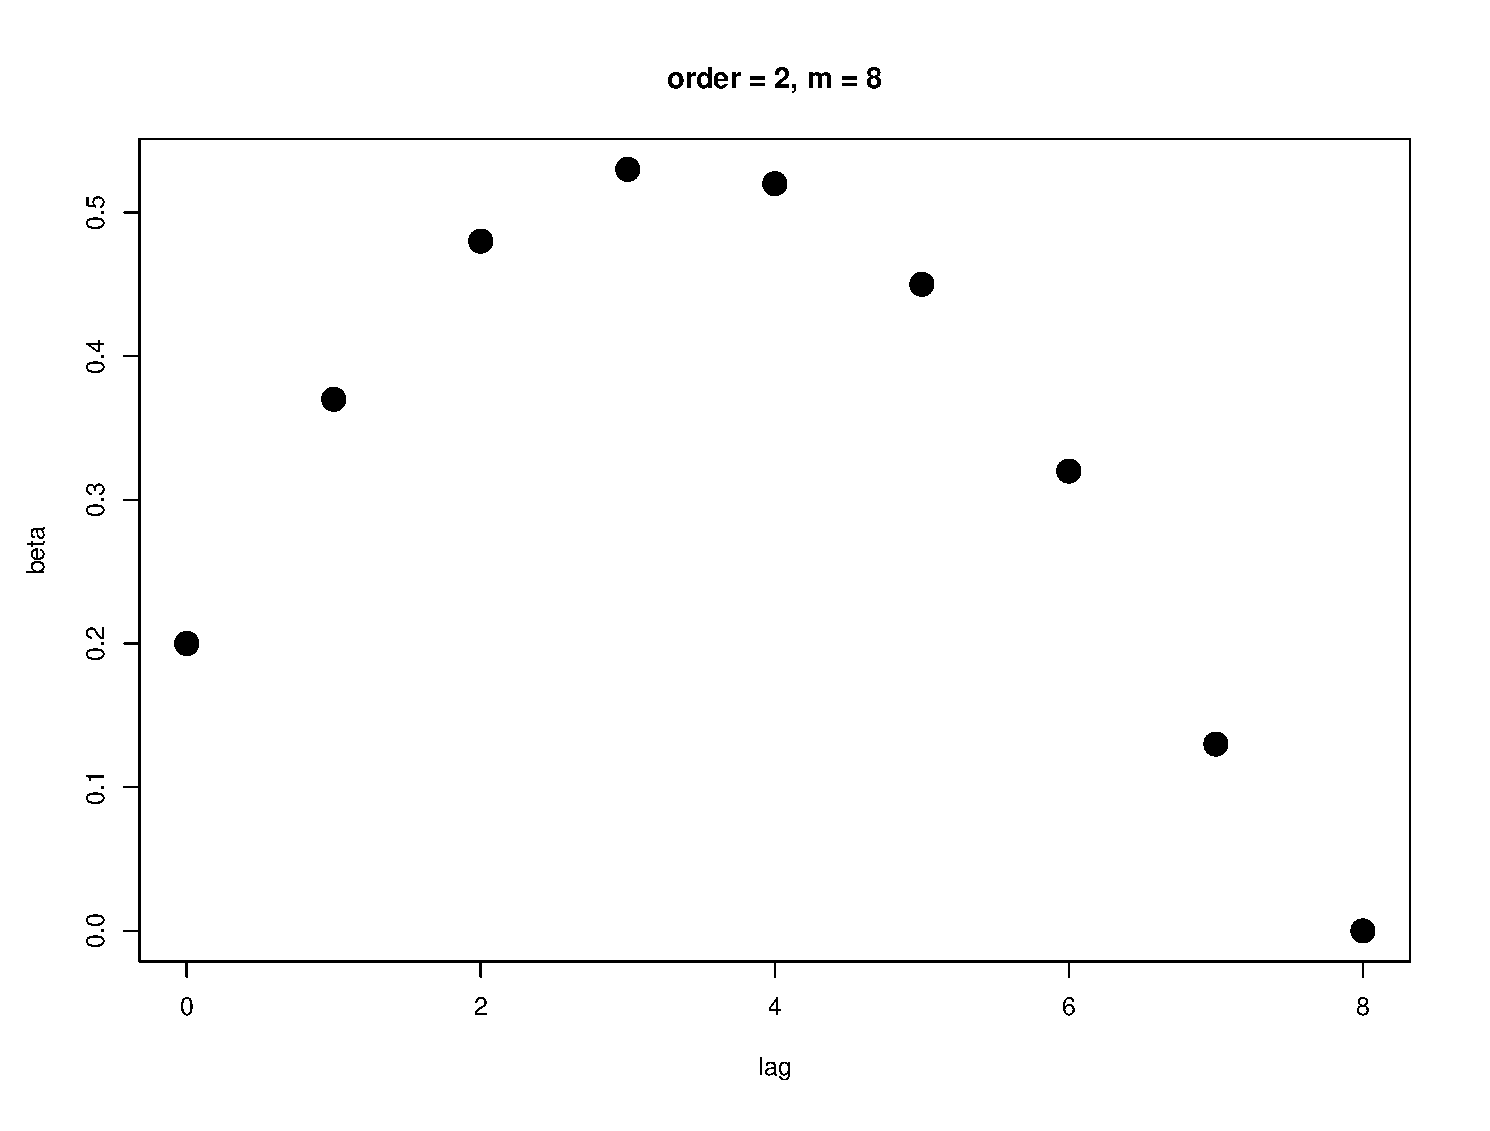
\includegraphics[width=\textwidth]{img/Polynom_2.eps}
\end{minipage}
\end{figure}
\end{frame}


%------------------------------------------------

\begin{frame}{Polynomial distributed lag}
\begin{itemize}
\item Almon-type transformation of \eqref{Almon1} for $m=8$ and $k=2$:
\begin{align} \nonumber
y_t & =  \alpha + k_0 x_t + (k_0 + k_1 + k_2)x_{t-1} + (k_0 + 2k_1 + 4k_2)x_{t-2} + \\ & + \dots + (k_0 + 8k_1 + 64k_2)x_{t-8}+u_t 
\\ \nonumber
y_t & = \alpha + k_0 (x_t + x_{t-1} + \dots + x_{t-8}) + \\ \nonumber & +  k_1(x_{t-1} + 2 x_{t-2} + \dots + 8 x_{t-8}) + \\ \nonumber & + k_2(x_{t-1} + 4x_{t-2} + \dots + 64x_{t-8}) = \\ 
y_t & = \alpha + k_0 \underbrace{\sum_{i=0}^8 x_{t-i}}_{W_{0t}} + k_1 \underbrace{\sum_{i=1}^8 i\, x_{t-i}}_{W_{1t}}  + k_2 \underbrace{\sum_{i=1}^8 i^2 x_{t-i}}_{W_{2t}}  + u_t\\
y_t & = \alpha + k_0 W_{0t} + k_1 W_{1t} + k_2 W_{2t} + u_t \label{eqpol3}
\end{align}
We estimate \eqref{eqpol3}, then calculate $\beta_i$ (lags 0 to 8) as in \eqref{eqpol2}\\
\dots note the reduction in estimated parameters (10 vs 4).
\end{itemize}
\end{frame}

%------------------------------------------------

\begin{frame}{Polynomial distributed lag}

\begin{itemize}
\item Method developed by Shirley Almon in the 60ies.
\item Equation \eqref{eqpol3} can be generalized: for $m$ lags, sums go to $m$, for higher order polynomials, we add more $W$-terms.
\vspace{0.3cm}
\item Advantages of this approach:
\begin{itemize}
\item Saves degrees of freedom
 \item Removes the problem of multicollinearity
 \item Does not affect the assumptions for $u$, because errors do not change during transformation
\end{itemize}
\vspace{0.3cm}
\item In EViews, transformation is slightly modified.
\item In R, routines are available.

\end{itemize}
\end{frame}

%------------------------------------------------
\section{Geometric distributed lag (Koyck) }
\begin{frame}{Geometric distributed lag (Koyck) }

IDL linear regression model: $y_t = f(x_t, x_{t-1}, x_{t-2}, \dots)$: 
\\ \vspace{0.3cm}
$ y_t = \alpha + \delta_0 x_t + \delta_1 x_{t-1} + \delta_2 x_{t-2} + \delta_3 x_{t-3} 
+ \dots + u_t$ \\ \vspace{0.3cm}
Assumption for the geometric $\delta_j$ weights:
\begin{itemize}
\item $ \delta_{j} = \gamma \rho^{\,j}$, \hspace{0.3cm} $0 < \rho < 1 $, $\hspace{0.3cm} j=0,1,2,\dots $\\
\smallskip
$|\rho|<1$ is a more general (valid) stability assumption.\\
$\left( j \textnormal{~is the lag operator here} \right)$\\
Sometimes, the assumption is written as $\delta_j = \delta_{j-1}\, \rho, \hspace{0.3cm} 0 < \rho < 1 $.
\end{itemize}
 
\vspace{0.3cm}
Instantaneous propensity (multiplier): $ \delta_0 = \gamma \rho^0 = \gamma$ 
\\ \vspace{0.3cm}
Long-run propensity (multiplier):
\\ \vspace{0.3cm}
$\delta_0+\delta_1+\dots=\gamma(1+\rho+\rho^2+\rho^3+\dots)=\frac{\gamma}{1-\rho}$

\end{frame}
%------------------------------------------------
\begin{frame}{Geometric distributed lag (Koyck) }
\textbf{Koyck transformation of the IDL model:}
\begin{align} 
y_t & = \alpha + \delta_0 x_t \,\,\,\,\,\,\,\, + \delta_1 x_{t-1} \,\,+ \delta_2 x_{t-2} + \dots + u_t \notag \\
\hline \notag \\ 
y_t & = \alpha + \gamma (\rho^0) x_t + \gamma\rho x_{t-1} + \gamma\rho^2 x_{t-2}+\dots + u_t \label{IDL} \\ 
y_{t-1} & = \alpha + \gamma x_{t-1} + \gamma\rho x_{t-2} + \gamma\rho^2 x_{t-3} + \dots+u_{t-1} \hspace{0.3cm} |\times \rho 
\\ \label{eqk3}
\rho y_{t-1} & = \alpha\rho + \gamma\rho x_{t-1} + \gamma \rho^2 x_{t-2} + \dots + \rho u_{t-1}
\end{align}
\centering Now, we subtract \eqref{eqk3} from \eqref{IDL}: \par
\begin{align}
y_t-\rho y_{t-1} & = \underbrace{\alpha(1-\rho)}_{\alpha_{0}}+\gamma x_t + \underbrace{u_t-\rho u_{t-1}}_{v_t}\\
y_t & = \alpha_0 + \gamma x_t + \rho y_{t-1} + v_t \label{Koyck}
\end{align}
\end{frame}

%------------------------------------------------
\begin{frame}{Geometric distributed lag (Koyck) }

IDL model: $\quad \,y_t = \alpha + \delta_0 x_t  + \delta_1 x_{t-1} + \delta_2 x_{t-2} + \dots + u_t $\\
\medskip
Koyck transf.: $y_t = \alpha_0 + \gamma x_t + \rho y_{t-1} + v_t$ \\
\medskip
Using the Koyck transformation, we can calculate parameters \\of the IDL model from the estimated model after Koyck transformation:\\
\medskip
$\quad \hat{\delta}_0 = \hat{\gamma}$ \\
\medskip
$\quad \hat{\delta}_j = \hat{\gamma} \, \hat{\rho}^{\,j} \,\, ; \,\, j = 1,2,3, \dots$ \\
\medskip
$\quad \hat{\alpha} = \frac{\hat{\alpha}_0}{1-\hat{\rho}}$\\
\medskip
Problems of the Koyck transformation:
\begin{itemize}
    \item in \eqref{Koyck}, regressor $y_{t-1}$ is not exogenous ($v_t=u_t-\rho u_{t-1}$)\\ \dots IVR will be discussed in Week 8
    \item $v_t=u_t-\rho u_{t-1}$ is not i.i.d.
\end{itemize}


\end{frame}
%------------------------------------------------

\begin{frame}{Rational distributed lag}
The geometric distributed lag is a special case of \\rational distributed lag (RDL) model:
\begin{align} \nonumber
y_t & = \alpha_0+\gamma x_t + \rho y_{t-1} + v_t \hspace{0.3cm} \textnormal{(geometric distributed lag)}\\\label{eqrat1} 
y_t & = \alpha_0+\gamma_0 x_t + \rho y_{t-1} +\gamma_1 x_{t-1} + v_t  \hspace{0.3cm} \textnormal{ (RDL)}
\end{align}
This can be shown by successive substitution ($|\rho| < 1$):
\begin{align}\nonumber
y_t & = \alpha + \gamma_0 (x_t + \rho x_{t-1} + \rho^2 x_{t-2}+\dots) \\ & + \gamma_1 (x_{t-1} + \rho x_{t-2} + \rho^2 x_{t-3}+\dots) + u_t \\ \nonumber
y_t & = \alpha + \gamma_0 x_t + (\rho \gamma_0 + \gamma_1) x_{t-1} + \rho (\rho \gamma_0 + \gamma_1) x_{t-2} +\\ & + \rho^2 (\rho \gamma_0 + \gamma_1) x_{t-3} + \dots + u_t \label{eqrat2}
\end{align}
After estimating \eqref{eqrat1}, we can calculate lag distributions for \eqref{eqrat2}

\end{frame}

%------------------------------------------------
\begin{frame}{Rational distributed lag}
RDL specification:\\
\medskip
$\quad y_t = \alpha_0+\gamma_0 x_t + \rho y_{t-1} +\gamma_1 x_{t-1} + v_t $\\
\medskip
can be used to calculate $\delta_h$ in the IDL model:\\
\medskip
$\quad y_t = \alpha + \delta_0 x_t  + \delta_1 x_{t-1} + \delta_2 x_{t-2} + \dots + u_t $\\
\medskip
With RDLs, impact propensity $\gamma_0 \equiv \delta_0$ can differ in sign from lagged coefficients. \\
\medskip
$\delta_h = \rho^{h-1}(\rho \gamma_0 + \gamma_1)$ corresponds to the $x_{t-h}$ variable for $h \geq 1$. \\
\smallskip
~ \dots $\delta_0$ may differ in sign from ``lags'', even if $\rho > 0$.\\
~ \dots for $\rho > 0$, $\delta_h$ doesn't change sign with growing $h \geq 1$. \\
\bigskip
Long-run propensity: $\textit{LRP} = \frac{\gamma_0 + \gamma_1}{1-\rho},$\\
\smallskip
where $|\rho| < 1$ $\> \Rightarrow$ the sign of LRP follows the sign of $(\gamma_0+\gamma_1)$. \\
\medskip
Also,  $u_t = v_t + \rho v_{t-1} + \rho^2 v_{t-2} + \cdots \> \>  MA(\infty)$
\end{frame}
%------------------------------------------------
\begin{frame}{IDL/Koyck and RDL -- summary}
$y_t = \alpha + \delta_0 x_t  + \delta_1 x_{t-1} + \delta_2 x_{t-2} + \delta_3 x_{t-3}+ \dots + u_t $\\
\bigskip
IDL/Koyck: $y_t = \alpha_0 + \gamma x_t + \rho y_{t-1} + v_t$\\
\smallskip
RDL: $\qquad \quad y_t = \alpha_0+\gamma_0 x_t + \rho y_{t-1} +\gamma_1 x_{t-1} + v_t $\\
\bigskip
\begin{table}
\centering
\caption{Koyck vs. RDL coefficients}
\label{Tab1}
\begin{tabular}{|l|c|c|}
\hline
  & IDL/Koyck & RDL \\
  \hline 
Impact multiplier & $\delta_0=\gamma~~~$ & $\delta_0=\gamma_0$ \\
\hline
Lagged multiplier (lag $h$) & $\delta_h = \gamma \rho^h$ & $\delta_h = \rho^{h-1}(\rho \gamma_0 + \gamma_1)$ \\
\hline 
LRP & $\frac{\gamma}{1-\rho}$ & $\frac{\gamma_0 + \gamma_1}{1-\rho}$\\
\hline
\end{tabular}
\end{table} 

\end{frame}
%------------------------------------------------
\section{PAM, AEH, Rational expectations}

\begin{frame}{Partial adjustment model}
Partial adjustment model (PAM) \\is based on two main assumptions:
\begin{enumerate}
\item LRM describes behavior of $y_t^{\ast}$, which is the unobserved, \\ 
expected/equilibrium/target/optimum value of $y_t$:
\begin{equation}
{y}_t^\ast = \alpha + \beta x_t + u_t  ~~~~~~~~  \label{eqpam1} 
\end{equation}
\item Between two time periods, $y_t$ follows the process:
\begin{equation}
y_t - y_{t-1} = \theta ( y_t^\ast-y_{t-1}), \hspace{0.5cm} 0 < \theta < 1 \label{eqpam2}
\end{equation}
Hence, the actual $\Delta y_t$ is only a fraction of the ``desirable'' change from $y_{t-1}$ to the optimum value of $y_t^\ast$.
\\ \dots in the special case of $\theta = 1$, $\Delta y_t$ leads to optimum.\\
\medskip
Note: \eqref{eqpam2} can be re-written as: $y_t= \theta {y}_t^\ast + (1-\theta)y_{t-1} $
\end{enumerate}

\end{frame}

%------------------------------------------------
\begin{frame}{Partial adjustment model}
Parameter estimation of PAM:
\begin{equation*}
{y}_t^\ast = \alpha + \beta x_t + u_t ~~~~~~~~~~~~~~~~~~~~~~~~~ \tag{\ref{eqpam1}}
\end{equation*}
\vspace{-0.6cm}
\begin{equation*}
y_t= \theta {y}_t^\ast + (1-\theta)y_{t-1}, \hspace{0.5cm} 0 < \theta < 1 \tag{\ref{eqpam2}}
\end{equation*}

\begin{enumerate}
\item Substitute for $y_t^\ast$ in \eqref{eqpam2} from \eqref{eqpam1}:\\
\begin{equation}
\begin{aligned}
y_t &= \alpha \theta &+~ \beta \theta x_t &+~ (1-\theta) y_{t-1} &+~ \theta u_t \label{eqpam3}\\
y_t &= \beta_0^{\prime} &+~ \beta_1^{\prime} x_t &+~ \beta_2^{\prime} y_{t-1} &+~ \theta u_t
\end{aligned}
\end{equation}
\item Estimate \eqref{eqpam3} and then calculate sought parameters of the PAM in \eqref{eqpam1} and \eqref{eqpam2}:\\
\smallskip
$\hat{\theta}= 1-\hat{\beta}_2^{\prime}$\\
\smallskip
$\hat{\alpha} =\hat{\beta}_0^{\prime}/\hat{\theta}$\\
\smallskip
$\hat{\beta} =\hat{\beta}_1^{\prime}/\hat{\theta}$
\end{enumerate}
\medskip
\small{\qquad Note that $\theta u_t$ can be independent of $y_{t-1}$ and i.i.d.}
\end{frame}

%------------------------------------------------
\begin{frame}{Partial adjustment model}
Parameter interpretation of PAM:

\begin{equation*}
\begin{aligned}
{y}_t^\ast &= \alpha + \beta x_t + u_t \\
y_t &= \theta {y}_t^\ast + (1-\theta)y_{t-1}, \hspace{0.5cm} 0 < \theta < 1 \\
\hline \\
y_t &= \alpha \theta +~ \beta \theta x_t +~ (1-\theta) y_{t-1} +~ \theta u_t \\
y_t &= \beta_0^{\prime} ~+~ \beta_1^{\prime} x_t +~ \beta_2^{\prime} y_{t-1} +~ \theta u_t
\end{aligned}
\end{equation*}
\medskip
Parameters:\\
\smallskip
\begin{itemize}
\item[$\theta~:\quad$] $\theta= (1-\beta_2^{\prime})$ is the adjustment coefficient; higher $\hat{\theta}$ indicates higher speed of adjustment towards equilibrium.\\
\smallskip
\item[$\beta_1^{\prime}:\quad$] impact multiplier (short-run marginal propensity)\\
\smallskip
\item [$\beta~:\quad$] $\beta =\beta_1^{\prime}/\theta$ is the long run multiplier.
\end{itemize}


\end{frame}

%------------------------------------------------

\begin{frame}{Adaptive expectations hypothesis}
Adaptive expectations hypothesis (AEH) \\ model is based on two main assumptions:
\bigskip
\begin{enumerate}
\item LRM describes behavior of $y_t$, as a function of ${x}_t^\ast$: the unobserved, 
expected/equilibrium/target/optimum value \\of $x_t$ 
(permanent income, potential output, etc.):
\begin{equation}
~~~~y_t = \alpha + \beta x_t^\ast + u_t.\label{eqare1}
\end{equation}
\item The unobserved ${x}_t^\ast$ process is defined as:
\begin{equation} \label{eqare2}
\begin{aligned}
x^\ast_t - x^\ast_{t-1} & = \phi( x_t - x_{t-1}^\ast), \hspace{0.5cm} 0 < \phi < 1\\
 &  \Downarrow \\
x_t^\ast & =  \phi x_t + (1-\phi) x^\ast_{t-1}.
\end{aligned}
\end{equation}
with $\phi=0$ for static expectations\\ and $~\phi=1$ for immediate adjustment.
\end{enumerate}
\footnotesize{Note: alternative $2^{nd}$ hypothesis: $x_t^\ast =  \phi x_{t-1} + (1-\phi) x^\ast_{t-1}. $}
\end{frame}
%------------------------------------------------
\begin{frame}{Adaptive expectations hypothesis}
Parameter estimation of AEH model:
\begin{equation}
y_t = \alpha + \beta x_t^\ast + u_t,~~ \tag{\ref{eqare1}}
\end{equation}
\begin{equation}
~~x_t^\ast =  \phi x_t + (1-\phi) x^\ast_{t-1} \tag{\ref{eqare2}}
\end{equation}
Successive substitution for $x_t^\ast$ from \eqref{eqare2} to \eqref{eqare1}: IDL process
\begin{equation}
y_t = \alpha + \beta \phi x_{t} 
    + \beta \phi (1-\phi)x_{t-1} + \beta \phi (1 - \phi)^2 x_{t-2} + \dots + u_t \label{eqare3}
 \end{equation}
After applying Koyck transformation, we get
\begin{equation} \label{eqare4}
\begin{aligned}
y_t &= \alpha \phi &+~ \beta \phi x_{t} &+~ (1-\phi) y_{t-1} &+~ v_t \\
y_t &= \beta_0^{\prime} &+~ \beta_1^{\prime} x_{t} &+~ \beta_2^{\prime} y_{t-1} &+~ v_t
\end{aligned}
\end{equation}
Estimate \eqref{eqare4}, then calculate parameters in \eqref{eqare1} and \eqref{eqare2}.
\smallskip
$\hat{\phi}= 1-\hat{\beta}_2^{\prime}$ ~~~($\phi$ is the ``adaptive expectations coefficient'')\\
\smallskip
$\hat{\alpha} =\hat{\beta}_0^{\prime}/\hat{\phi}$\\
\smallskip
$\hat{\beta} =\hat{\beta}_1^{\prime}/\hat{\phi}$ ~~~~~($\beta_1^{\prime}$ and $\beta$ are the SR and LR propensities )\\
\smallskip
\footnotesize{\qquad Note: Both problems of Koyck-transformed model estimation apply.}
\end{frame}
%------------------------------------------------

\begin{frame}{Koyck, PAM, AEH: regression of $y_t$ on $x_t$ and $y_{t-1}$}
The same underlying regression model (statistical form) is used:

\begin{itemize}
\item The Koyck transformation:\\
$y_t = \alpha_0 + \gamma x_t + \rho y_{t-1} + v_t$\\
\smallskip
\item The Partial adjustment model (PAM):\\
$y_t = \alpha \theta + \beta \theta x_t + (1-\theta) y_{t-1} + \theta u_t$\\
\smallskip
\item The Model with adaptive expectations (AEM):\\
$y_t = \alpha \phi + \beta \phi x_{t} + (1-\phi) y_{t-1} + v_t $\\

\end{itemize}
\vspace{0.3cm}
We can make three different interpretations from one estimated equation.\\
\vspace{0.3cm}
Of course, not all interpretations are always relevant, we must choose according to application and test assumptions.
\end{frame}
%------------------------------------------------
\begin{frame}{Koyck, PAM, AEH: regression of $y_t$ on $x_t$ and $y_{t-1}$}
\textbf{Example:} Model for $c_t \leftarrow f(x_t,x_{t-1},x_{t-2},\dots)$:\\
private consumption $(c_t)$ as a function of disposable income $(x_t)$.\\
Same estimated model for Koyck, PAM, AEH:
\begin{equation*}
\begin{aligned}
\hat{c}_t & = &1,038~&+ &0.404 x_t~ &+ &0.501 c_{t-1} \\
\textnormal{\textbf{Koyck:}} \,\,\, \hat{c}_t & = &\hat{\alpha}_0~&+ &\hat{\gamma} x_t~ &+ &\hat{\rho} c_{t-1} 
\end{aligned}
\end{equation*}

Koyck: IDL, geometric decay in $\delta$ parameters assumed:
\begin{itemize}
\item $\hat{\rho}=0.501$
\smallskip
\item $\hat{\alpha}_0 = 1,038 = \hat{\alpha}(1-\hat{\rho}) = \hat{\alpha}(1-0.501) 
\Rightarrow \hat{\alpha}= \frac{1,038}{0.499}=2,080$
\item $\hat{\delta}_j = \hat{\gamma} \hat{\rho}^{\,j}=0.404 \times 0.501^{\,j}$
\smallskip
\item $\textit{LRP}=\frac{\hat{\gamma}}{1-\hat{\rho}}= \frac{0.404}{0.499} \doteq 0.81 $
\smallskip
\item IDL: $\hat{c}_t = 2,080 + \underbrace{0.404}_{\hat{\gamma} \hat{\rho}^{0}} x_t + \underbrace{0.202}_{\hat{\gamma} \hat{\rho}} x_{t-1} 
+ \underbrace{0.101}_{\hat{\gamma} \hat{\rho}^{2}} x_{t-2} + \dots$
\end{itemize}
\end{frame}

%------------------------------------------------

\begin{frame}{Koyck, PAM, AEH: regression of $y_t$ on $x_t$ and $y_{t-1}$}
\textbf{Example} continued:
\begin{equation*}
\begin{aligned}
\hat{c}_t & = &1,038~&+ &0.404 x_t~ &+ &0.501 c_{t-1} \\
\textnormal{\textbf{PAM:}} \,\,\, \hat{c}_t& = &\hat{\alpha} \hat{\theta}~&+ &\hat{\beta} \hat{\theta} x_t~&+ &(1-\hat{\theta}) c_{t-1} 
\end{aligned}
\end{equation*}

\begin{itemize}
\item $(1-\hat{\theta})=0.501 \Rightarrow \hat{\theta} = 0.499$
\smallskip
\item $\hat{\alpha} \hat{\theta} = 1,038 \Rightarrow \hat{\alpha}= \frac{1,038}{0.499}=2,080$
\item $\hat{\beta} \hat{\theta} = ~ 0.404 \Rightarrow \hat{\beta}= \frac{0.404}{0.499} \doteq 0.81$
\bigskip
\item PAM: $\hat{c}_t^{\ast} = 2,080 + 0.81 x_t$\\
\smallskip
$c_t - c_{t-1} = 0.499 \cdot (c_t^{\ast}-c_{t-1})$
\bigskip
\item If $c_t$ has a prominent inertia and $\Delta c_t$ significantly follows changes in habits, we might use the PAM approach.
\end{itemize}
\end{frame}

%------------------------------------------------

\begin{frame}{Koyck, PAM, AEH: regression of $y_t$ on $x_t$ and $y_{t-1}$}
\textbf{Example} continued:
\begin{equation*}
\begin{aligned}
\hat{c}_t & = &1,038~&+ &0.404 x_t~ &+ &0.501 c_{t-1} \\
\textnormal{\textbf{AEH:}} \,\,\, \hat{c}_t& = &\hat{\alpha} \hat{\phi}~&+ &\hat{\beta} \hat{\phi} x_t~&+ &(1-\hat{\phi}) c_{t-1} 
\end{aligned}
\end{equation*}

\begin{itemize}
\item $(1-\hat{\phi})=0.501 \Rightarrow \hat{\phi} = 0.499$
\smallskip
\item $\hat{\alpha} \hat{\phi} = 1,038 \Rightarrow \hat{\alpha}= \frac{1,038}{0.499}=2,080$
\item $\hat{\beta} \hat{\phi} = ~ 0.404 \Rightarrow \hat{\beta}= \frac{0.404}{0.499} \doteq 0.81$
\bigskip
\item AEH: $\hat{c}_t = 2,080 + 0.81 x_t^{\ast}$\\
\smallskip
$~~~~~~~\,x_t^{\ast} = 0.499 x_t + 0.501 x_{t-1}^{\ast}$
\bigskip
\item If $c_t$ if formed as a function of expected (e.g. permanent) income, we might prefer AEH.
\end{itemize}
\end{frame}

%------------------------------------------------
\begin{frame}{Rational expectations}
\begin{itemize}
\item Rational expectations
$$\mathbf{E}_{t-1}(x_t)=a_0+a_1 x_{t-1} + b_1 z_{1,t-1}+b_2 z_{2, t-2}+\dots$$
$\mathbf{E}_{t-1}(x_t)$: expected value of $x_t$ at time $t-1$\\
$z_{k,t-j}$: exogenous variables with impact on $\mathbf{E}_{t-1}(x_t)$\\
\vspace{0.3cm}
We put $x_t^\ast = \mathbf{E}_{t-1}(x_t)$ into \eqref{eqare1}: $y_t = \alpha + \beta x_t^\ast + u_t$\\
\vspace{0.3cm}
We assume that agents:
\begin{itemize}
\item know all relevant information
\item know how to use this information
\end{itemize}
\vspace{0.3cm}
Agents can make prediction errors ($v_t$), so: $$x_t=x^\ast_t+v_t $$
\end{itemize}
\end{frame}

%------------------------------------------------

\begin{frame}{Rational vs. adaptive expectations}
Under rational expectations:
\vspace{0.3cm}
\begin{itemize}
\item Expected value of  prediction errors $[v_t = x_t - x^\ast_t]$ must be zero. If they were systematically different from zero, rational agents would immediately adjust their forecasting methods accordingly.
\vspace{0.3cm}
\item $[v_t = x_t - x^\ast_t]$ prediction error must be uncorrelated with any information available when the prediction is made $(t-1)$. If not, this would imply that the forecaster has not made use of all available information.
\vspace{0.3cm}
\item These properties can be used for testing the rational expectations hypothesis in different applications \\(e.g. through ex-post simulated dynamic forecasts).
\end{itemize}
\end{frame}

%------------------------------------------------

\begin{frame}{Some economic application that use expectations}
\begin{itemize}
\item Philips curve (Expectations-augmented Phillips curve)
\item Efficient market hypothesis (EMH)
\item Consumption function - Permanent income hypothesis
\end{itemize}
\end{frame}

%------------------------------------------------

\section{FWL theorem - repetition from BSc courses}
\begin{frame}{FWL theorem - repetition from BSc courses}
Frisch and Waugh in the 30-ies: detrending \\
Lovell in the 60-ies: deseasonalizing
\begin{itemize}
\item Example: Spurious regression with trend-stationary series: e.g. Regression of the US GDP on salmon production in Norway
\begin{block}{Solution (identical $\hat{\beta}_2$ estimates) }
M1: $\textit{gdp}_t = \beta_0 + \beta_1 \textit{year}_t + \beta_2 \textit{salmon}_t + u_t$\\
M2: $\textit{gdp.detrended}_t = \beta_2 \textit{salmon.detrended}_t + u_t$\\
M2: $\textit{gdp.detrended}_t = \beta_0 + \beta_1 \textit{year}_t + \beta_2 \textit{salmon}_t + u_t$\\
M4: $\textit{gdp}_t = \beta_2 \textit{salmon.detrended}_t + u_t$
\end{block}
\item Note that $\beta_0$, $\beta_1$ and $u_t$ may differ among equations.
\end{itemize}
\end{frame}

%------------------------------------------------

\begin{frame}{FWL theorem}
\begin{itemize}
\item Partitioned regression
\begin{equation} \label{FWLpart}
\bm{y} = \bm{X}  \bm{\beta} + u = 
\bm{X}_1 \bm{\beta}_1 + \bm{X}_2 \bm{\beta}_2 + \bm{u}
\end{equation}
\item Projection matrices and residual makers
\begin{align*}
\bm{P}  & = \bm{X}(\bm{X}^{\prime}\bm{X})^{-1}\bm{X}^{\prime}, \hspace{0.5cm}
& \bm{M} & = \bm{I} - \bm{P}\\
\bm{P}_1 & = \bm{X}_1(\bm{X}_1^{\prime}\bm{X}_1)^{-1}\bm{X}_1^{\prime}, \hspace{0.5cm} & \bm{M}_1 & =\bm{I}-\bm{P}_1\\
\bm{P}_2 & = \bm{X}_2 (\bm{X}_2^{\prime}\bm{X}_2)^{-1}\bm{X}_2^{\prime}, \hspace{0.5cm} & \bm{M}_2 & =\bm{I}-\bm{P}_2
\end{align*}
\item Some properties
\begin{align*}
\bm{P}\bm{P}_1 & = \bm{P}_1, \hspace{0.2cm} \bm{P}\bm{X}_1 = \bm{X}_1~~ \textnormal{($\bm{X}_1$ is in the span ($\bm{X}$))}\\
\bm{P}\bm{P}_1 & = (\bm{P}_1\bm{P})^{\prime}=\bm{P}_1\bm{P}=\bm{P}_1\\
\bm{M}\bm{M}_1 & = (\bm{M}_1\bm{M})^{\prime}=\bm{M}_1\bm{M}=\bm{M} \\
\bm{M}_1\bm{X}_1 & = \bm{0}, \quad \bm{X}_2^{\prime}\bm{M}=\bm{0} \\
\end{align*}
\end{itemize}
\end{frame}

%------------------------------------------------

\begin{frame}{FWL theorem}
M1: $\textit{gdp}_t = \beta_0 + \beta_1 \textit{year}_t + \beta_2 \textit{salmon}_t + u_t$\\
$ \bm{y} = \bm{X}_1 \bm{\beta}_1 + \bm{X}_2 \bm{\beta}_2 + \bm{u}=\bm{X} \bm{\beta} + u$\\
\vspace{0.5cm}
M2: $\textit{gdp.detrended}_t = \beta_2 \textit{salmon.detrended}_t + u_t$\\
$\bm{M}_1 \bm{y} = \bm{M}_1\bm{X}_2\bm{\beta}_2+\bm{u}$\\
\vspace{0.5cm}
M3: $\textit{gdp.detrended}_t = \beta_0 + \beta_1 \textit{year}_t + \beta_2 \textit{salmon}_t + u_t$\\
$\bm{M}_1 \bm{y} = \bm{X}_1 \bm{\beta}_1 + \bm{X}_2\bm{\beta}_2+\bm{u}$\\
\vspace{0.5cm}
M4: $\textit{gdp}_t = \beta_2 \textit{salmon.detrended}_t + u_t$ \\
$\bm{y} = \bm{M}_1\bm{X}_2 \bm{\beta}_2 +\bm{u}$\\
\end{frame}

%------------------------------------------------

\begin{frame}{FWL theorem}

\textbf{FWL theorem \& applications}

\begin{enumerate}
\item Estimates of $\beta_2$ for a partioned model \eqref{FWLpart} in all M1 - M4 models are the same
\item Residuals from M1, M2, M3 are the same
\end{enumerate}
\vspace{0.5cm}
\textbf{Lemma}: Based on properties of projection matrices and residual makers, we can show that  $\bm{\hat{\beta}}_2$ estimators in all four (M1 to M4) specifications can be expressed as: 
$$\bm{\hat{\beta}}_2 = (\bm{X}_2^{\prime}\bm{M}_1 \bm{X}_2)^{-1}\bm{X}_2^{\prime}\bm{M}_1\bm{y} $$

\textbf{Application:} deseasonalizing, centered coefficient of determination, interchangeability of reference categories (e.g. quarterly dummies), simplification of many proofs in econometrics
\end{frame}

%------------------------------------------------
%
\begin{frame}{FWL theorem (detrending)}
$$\bm{y} ~~=~~ 
\bm{X}\hat{\bm{\beta}} + \hat{\bm{u}} ~~ = 
~~ 
\bm{Py} + \bm{My} ~~ =
~~ 
\bm{X}_1\hat{\bm{\beta}}_1+\bm{X}_2\hat{\bm{\beta}}_2+\bm{My}$$
\begin{block}{Skeleton of the proof (for M1 equation):}
\vspace{-0.3cm}
\begin{align*}
\bm{y} & = \bm{X}_1 \bm{\hat{\beta}}_1+ \bm{X}_2\bm{\hat{\beta}}_2+\bm{M}\bm{y} \quad
| \quad \bm{X}^{\prime}_2\bm{M}_1 \times \\
\bm{X}^{\prime}_2\bm{M}_1\bm{y} & = \underbrace{\bm{X}^{\prime}_2\underbrace{\bm{M}_1\bm{X}_1}_{\bm{0}} \bm{\hat{\beta}}_1}_{\bm{0}}+ \bm{X}^{\prime}_2\bm{M}_1\bm{X}_2\bm{\hat{\beta}}_2+ \underbrace{\underbrace{\bm{X}^{\prime}_2\underbrace{\bm{M}_1\bm{M}}_{\bm{M}}}_{\bm{0}}\bm{y}}_{\bm{0}}\\
\bm{X}^{\prime}_2\bm{M}_1\bm{y} & \! = \! \bm{X}^{\prime}_2\bm{M}_1\bm{X}_2\bm{\hat{\beta}}_2 \Rightarrow \! \bm{\hat{\beta}}_2 = (\bm{X}^{\prime}_2\bm{M}_1\bm{X}_2)^{-1}\bm{X}^{\prime}_2\bm{M}_1\bm{y}\Rightarrow \textnormal{QED}
\end{align*}
\end{block}
\end{frame}
%------------------------------------------------
\end{document}